\section{Introducción}

\subsection{Área temática}
\begin{frame}{Área temática}
	Este trabajo se basa en 5 pilares teóricos:
	\medskip
	\begin{itemize}[<*>]
		\item Sistemas de Recomendación.
		\item Sitios de Community Question Answering (CQA).
		\item Medidas de similaridad.
		\item Ensamble de Clustering.
		\item Big Data.
	\end{itemize}
\end{frame}

\begin{frame}{Área temática II}
	\textbf{Area temática}
	\medskip
	\begin{itemize}
		\item Miles de nuevas preguntas son formuladas diariamente en sitios de CQA como Yahoo! Answers, Stackexchange, Stackoverflow, o Quora.
		\item Muchas de las preguntas no están respondidas correctamente o no tienen respuestas.
		\begin{itemize}[<*>]
			\item Pequeño número de expertos entre la gran población de usuarios.
			\item La pregunta es difícil de ubicar dentro del sitio.
			\item Respuestas maliciosas.
		\end{itemize}
		\item Es de interés buscar si esa misma pregunta ha sido formulada por otro usuario previamente, y que tenga la respuesta buscada.
		\item Preguntas que poseen la misma respuestas están formuladas de forma diferente en el sentido léxico. \\
		\begin{center}
			\begin{footnotesize}
				\textit{¿Cómo elijo una revista para publicar mi artículo?} y \textit{¿Dónde publico mi artículo?}
			\end{footnotesize}
		\end{center}
	\end{itemize}
 \end{frame}

\begin{frame}{Área temática III}
	\textbf{Area temática (cont.)}
	\medskip
	\begin{itemize}
		\item Es necesaria una medida de similaridad que tenga en cuenta características léxicas y semánticas.
		\item La tarea de recomendar preguntas similares en sitios de CQA puede ser llevada a cabo por un RS.
		\item Se diseñó e implementó una arquitectura Big Data para crear una medida de similaridad que alimente a un RS para sitios de CQA.
	\end{itemize}
\end{frame}

\subsection{Tema específico}
\begin{frame}[allowframebreaks]{Tema específico}
	Pipeline para un RS basado en contenido de CQA y en una nueva medida de similaridad.
	\medskip
	\begin{figure}
		\centering
		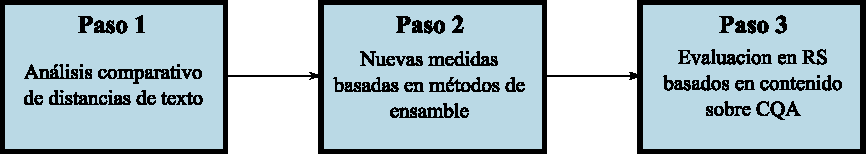
\includegraphics[width=0.7\linewidth]{../5_introduccion/imagenes/pipeline}
		\label{fig:pipeline}

		\bigskip

		Este trabajo se enfoca en el \textbf{Paso 2} del pipeline.

		\framebreak

		Considerando el conjunto completo de datos Quora (\(404301\) pares de preguntas, es decir, \(808602\) preguntas totales), deberíamos realizar:

		\bigskip $\frac{n(n+1)}{2} = 326919001503$ calculos de distancias, donde $n = 808602$

		\bigskip
		\bigskip

		Esta situación plantea la necesidad de considerar una arquitectura Big Data.
	\end{figure}
\end{frame}

\subsection{Objetivo general}
\begin{frame}{Objetivo general}
	\begin{tcolorbox}[colback=blue!5,colframe=blue!40!black,title=Objetivo general]
	El presente trabajo de investigación tiene como objetivo construir una \textbf{arquitectura Big Data} que incluye la posibilidad de ser aplicada a grandes conjuntos de datos en el ámbito de \textbf{CQA} y, a partir de esta arquitectura, implementar, evaluar y realizar un \textbf{análisis comparativo con el estado del arte de una nueva medida de similaridad entre textos} que pueda ser utilizada en \textbf{Sistemas de Recomendación}.
	\end{tcolorbox}
\end{frame}

\subsection{Objetivos específicos}
\begin{frame}{Objetivos específicos}
	\begin{tcolorbox}[colback=blue!5,colframe=blue!40!black,title=Objetivos específicos]
		\begin{footnotesize}
			\begin{itemize} [<+>]
				\item Diseñar y desarrollar una \textbf{arquitectura Big Data} para cálculo de similaridad en grandes volúmenes de datos.
				\item Identificar \textbf{medidas de similaridad de texto} existentes y un método efectivo de aplicación de las mismas en grandes volúmenes de datos.
				\item \textbf{Proponer una nueva medida} que permita integrar las medidas de similaridad del estado del arte mediante una arquitectura de software basada en Big Data.
				\item \textbf{Evaluar el comportamiento} de una medida de similaridad de texto del estado del arte respecto al manejo del volumen, variedad, velocidad y veracidad inherentes a grandes volúmenes de datos.
				\item \textbf{Brindar conclusiones, pautas y recomendaciones} para trabajar con medidas de comparación de textos en grandes volúmenes de datos en sitios de CQA utilizando arquitecturas basadas en Big Data.
			\end{itemize}
		\end{footnotesize}
	\end{tcolorbox}
\end{frame}